\begin{frame}
\frametitle{Mini-Project: Generating a Weather Report}

\begin{columns}

	\begin{column}{0.6\textwidth}
		The National Weather Service makes available an API
		providing critical forecasts, alerts, observations,
		and other weather data products.
		
		\vspace{12pt}
		
		Let's design and implement an NLG system
		that takes local forecast data as input,
		and produces a textual report
		of the most relevant features in the forecast.
	\end{column}
	
	\begin{column}{0.4\textwidth}
		\centering
		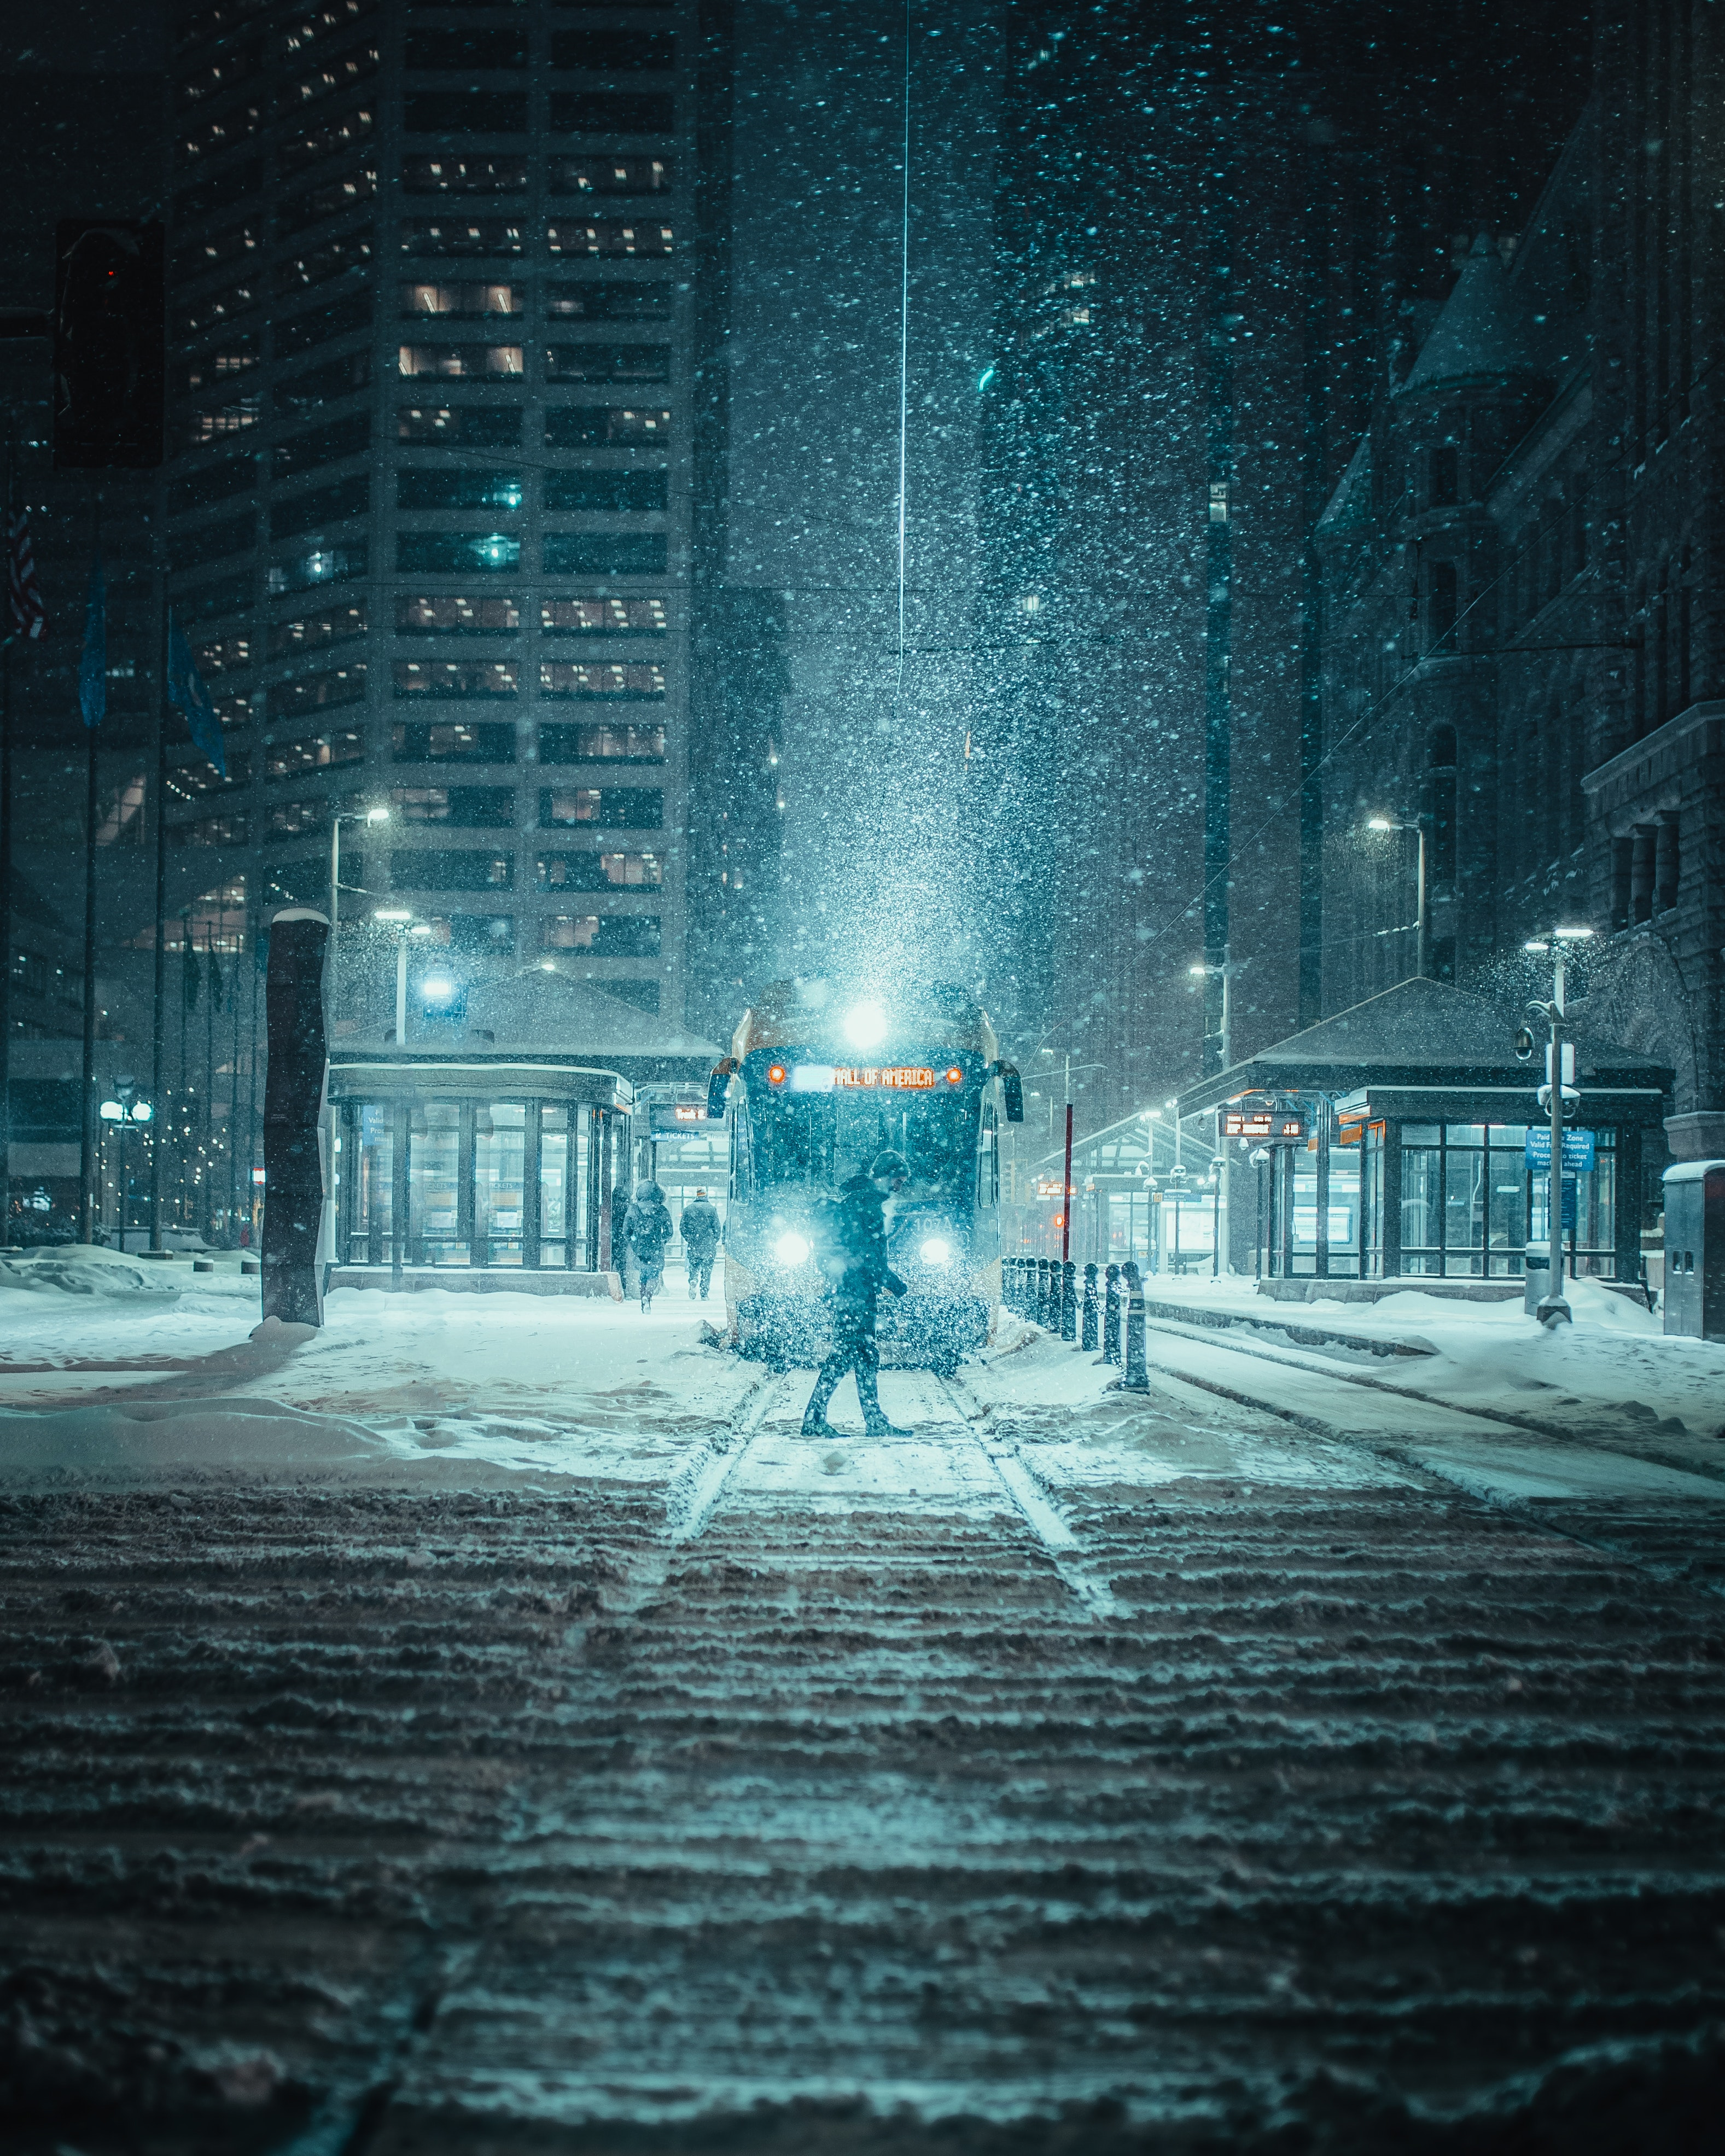
\includegraphics[width=0.8\textwidth]{pexels-josh-hild-2422497}
	\end{column}

\end{columns}

\vspace{12pt}

Documentation: \href{https://www.weather.gov/documentation/services-web-api}{https://www.weather.gov/documentation/services-web-api}

API: \href{https://api.weather.gov/}{https://api.weather.gov/}


\end{frame}